\documentclass[final, 10pt]{beamer}

\usepackage[scale=1.24]{beamerposter} % Use the beamerposter package for laying out the poster
\usepackage{lmodern}

\usetheme{confposter} % Use the confposter theme supplied with this template

\setbeamercolor{block title}{fg=blue,bg=white} % Colors of the block titles
\setbeamercolor{block body}{fg=black,bg=white} % Colors of the body of blocks
\setbeamercolor{block alerted title}{fg=white,bg=dblue!70} % Colors of the highlighted block titles
\setbeamercolor{block alerted body}{fg=black,bg=dblue!10} % Colors of the body of highlighted blocks
% Many more colors are available for use in beamerthemeconfposter.sty

%-----------------------------------------------------------
% Define the column widths and overall poster size
% To set effective sepwid, onecolwid and twocolwid values, first choose how many columns you want and how much separation you want between columns
% In this template, the separation width chosen is 0.024 of the paper width and a 4-column layout
% onecolwid should therefore be (1-(# of columns+1)*sepwid)/# of columns e.g. (1-(4+1)*0.024)/4 = 0.22
% Set twocolwid to be (2*onecolwid)+sepwid = 0.464
% Set threecolwid to be (3*onecolwid)+2*sepwid = 0.708

\newlength{\sepwid}
\newlength{\onecolwid}
\newlength{\twocolwid}
\newlength{\threecolwid}
\setlength{\paperwidth}{48in} % A0 width: 46.8in
\setlength{\paperheight}{36in} % A0 height: 33.1in
\setlength{\sepwid}{0.024\paperwidth} % Separation width (white space) between columns
\setlength{\onecolwid}{0.22\paperwidth} % Width of one column
\setlength{\twocolwid}{0.464\paperwidth} % Width of two columns
\setlength{\threecolwid}{0.708\paperwidth} % Width of three columns
\setlength{\topmargin}{-0.5in} % Reduce the top margin size
%-----------------------------------------------------------

\usepackage{graphicx}  % Required for including images
\graphicspath{ {figures/} }
\usepackage{booktabs} % Top and bottom rules for tables
\usepackage{amsmath,mathtools,bbm}

%----------------------------------------------------------------------------------------
%	TITLE SECTION 
%----------------------------------------------------------------------------------------

\title{Quantifying Uncertainty in Mass Spectrometry Based Spatial Proteomics} % Poster title

\author{Oliver M. Crook, Laurent Gatto, Paul D.W.Kirk, Kathryn Lilley} % Author(s)

\institute{Cambridge Centre for Proteomics, Computational Proteomics Unit, MRC Biostatistics Unit, University of Cambridge} % Institution(s)

%----------------------------------------------------------------------------------------

\begin{document}

\addtobeamertemplate{block end}{}{\vspace*{2ex}} % White space under blocks
\addtobeamertemplate{block alerted end}{}{\vspace*{2ex}} % White space under highlighted (alert) blocks

\setlength{\belowcaptionskip}{2ex} % White space under figures
\setlength\belowdisplayshortskip{2ex} % White space under equations

\begin{frame}[t] % The whole poster is enclosed in one beamer frame

\begin{columns}[t] % The whole poster consists of three major columns, the second of which is split into two columns twice - the [t] option aligns each column's content to the top

\begin{column}{\sepwid}\end{column} % Empty spacer column

\begin{column}{\onecolwid} % The first column

%----------------------------------------------------------------------------------------
%	INTRODUCTION
%----------------------------------------------------------------------------------------

\begin{block}{Introduction}

  \begin{itemize}
  \small{\item The sub-cellular localisation of proteins is crucial to execute their intended function, and aberrant localisations are a hallmark of many diseases, including cancer and obesity.
  \item State-of-the art experimental procedures exist, that rely on 
  separation of cellular content and high accuracy mass spectrometry, to determine protein localisations. 
  \item In the \textit{hyper}LOPIT protocol, organelles and macro-molecular complexes are characterised by density-specific profiles along a gradient. 
  \item Quantitative protein profiles that match the organelle profiles along the gradient are produced using high throughput mass spectrometry (MS).}
  \item Organelle profiles can be modelled using non-parametric Bayesian techniques such a Gaussian Process regression.
  \end{itemize}

  % ------------------------------------------------

  \begin{figure}
    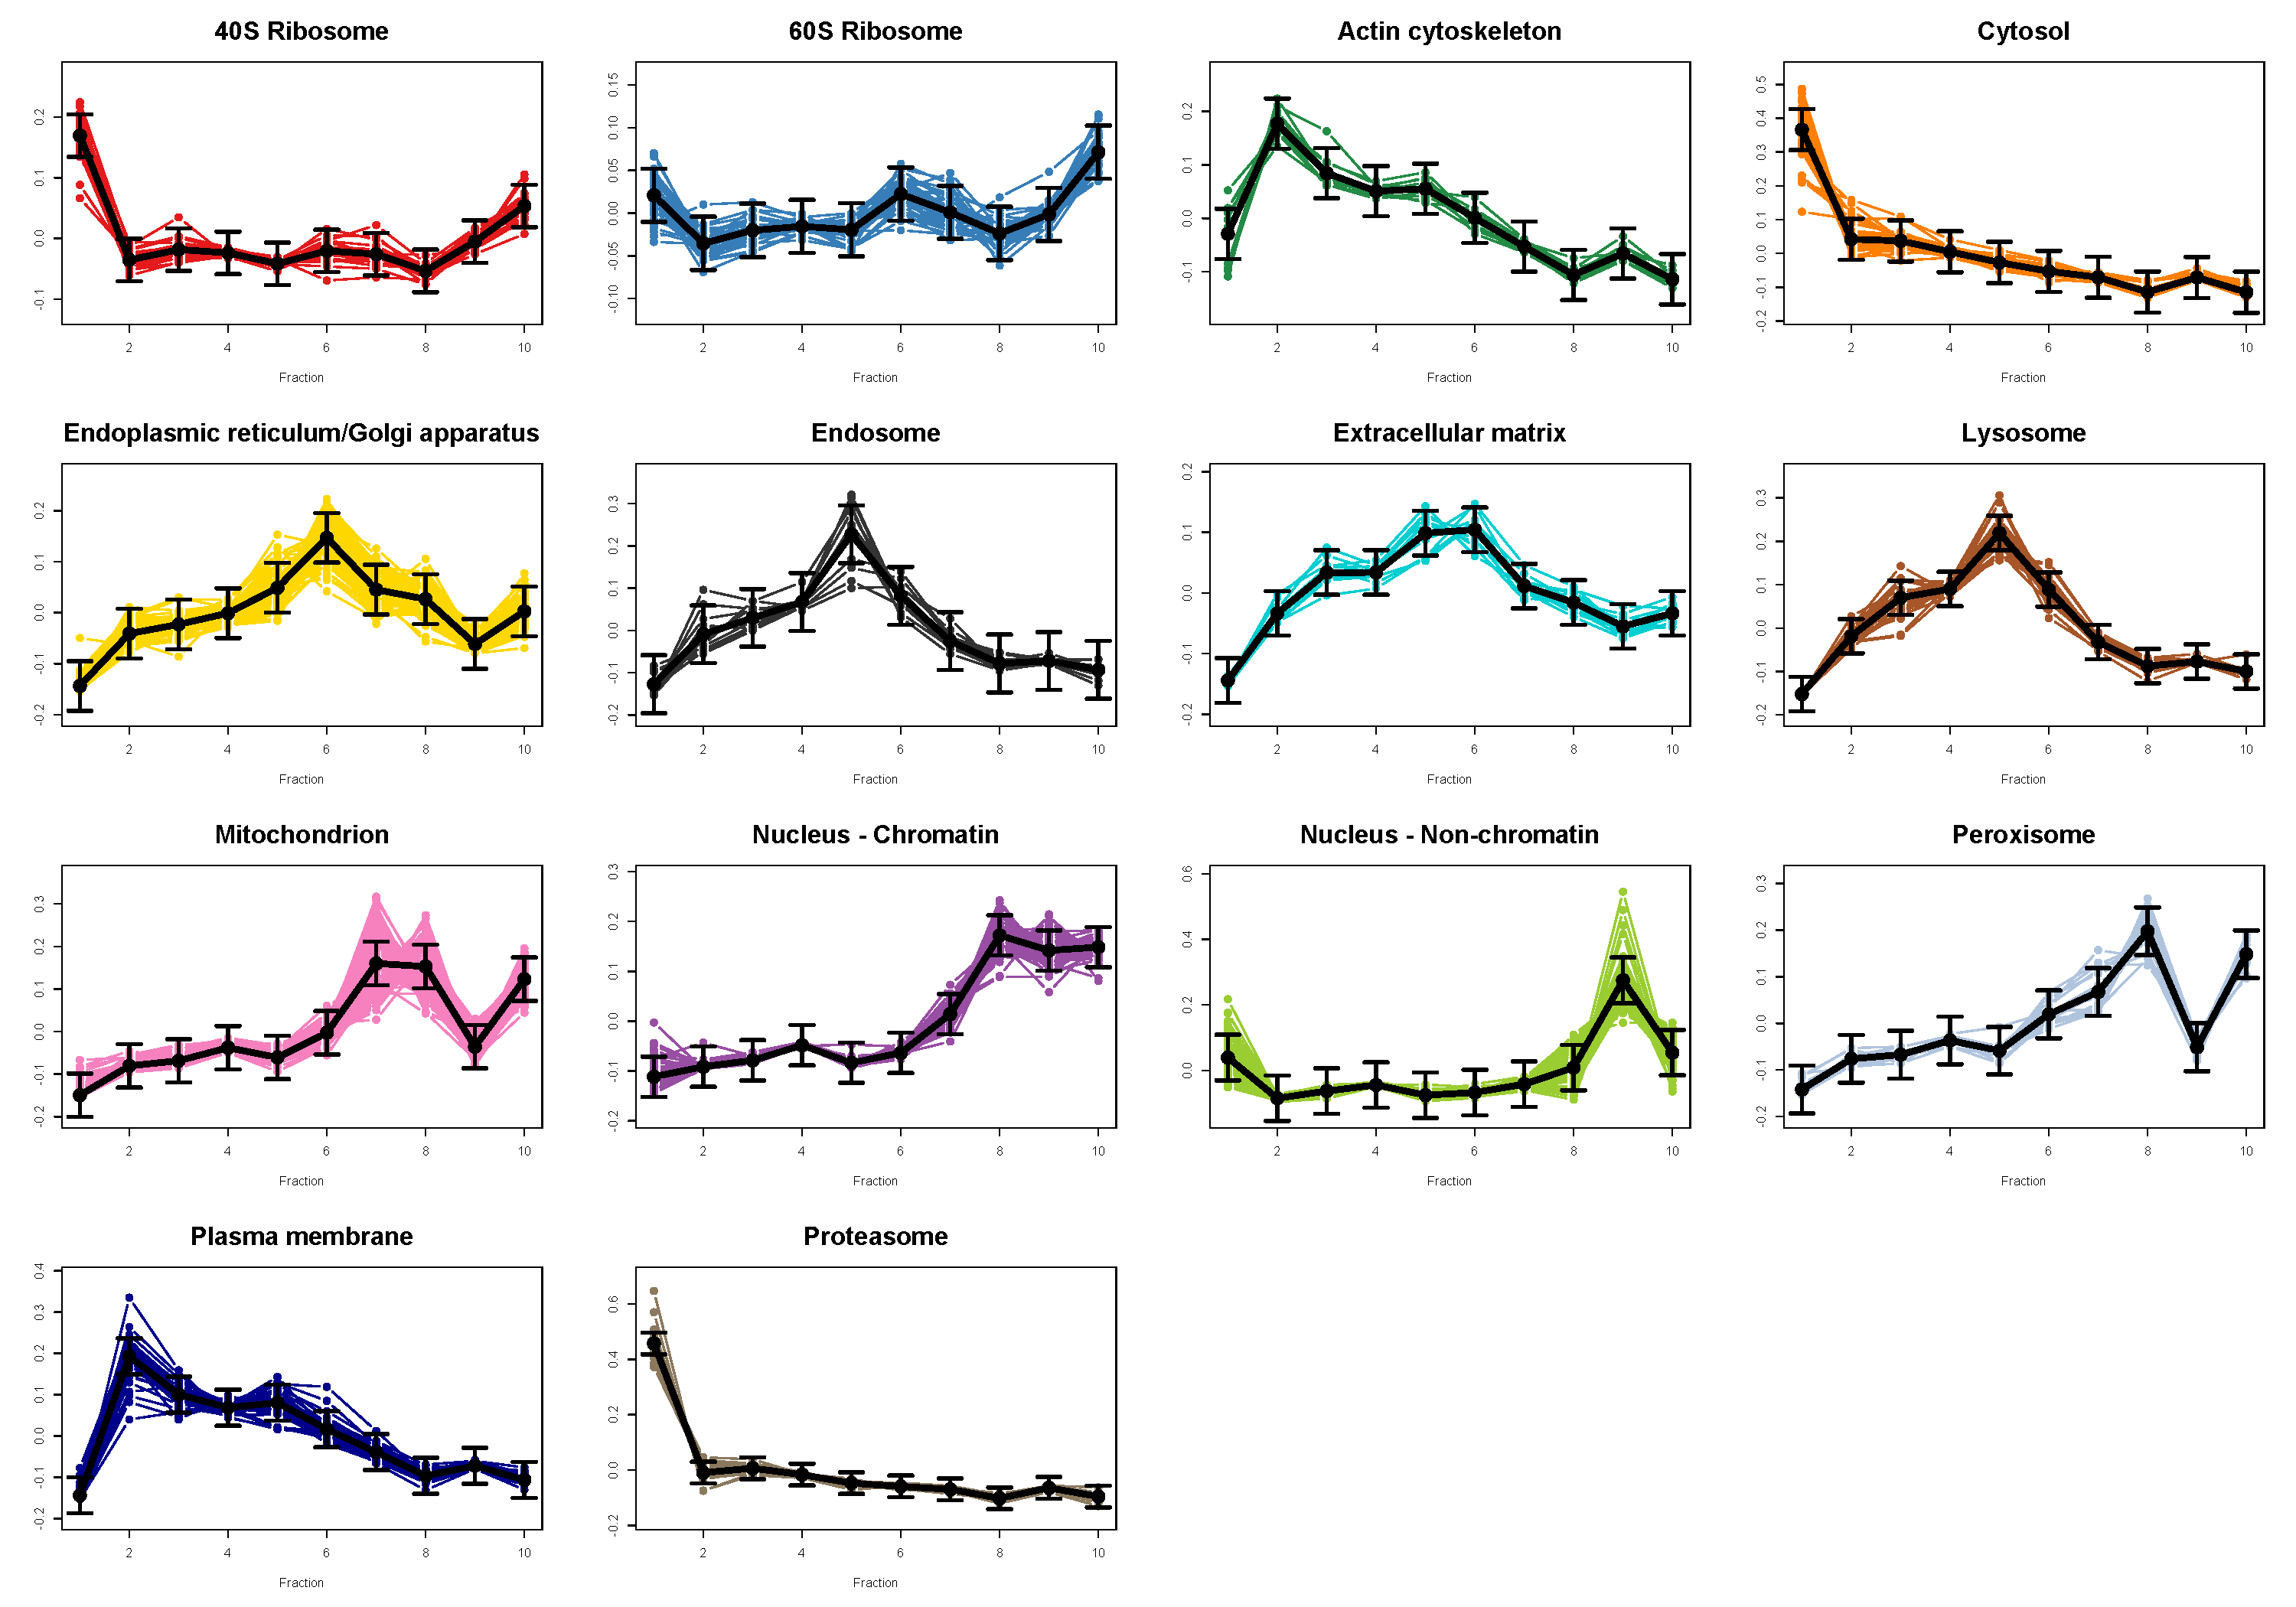
\includegraphics[width=1\linewidth]{GPallprofiles}
    \caption{ Proteins with known localisation to organelles and macro-molecular complexes in a mouse pluripotent embryonic stem cell dataset are modelled using Gaussian processes. The Gaussian process regression model captures the non-linearity of each unique profile.}
  \end{figure}

  % ----------------------------------------------------------------------------------------
  \begin{itemize}
  \small{\item Previously, supervised machine learning algorithms have been employed to create classifiers that make protein-organelle assigments. 
  \item However, proteins can be distributed amongst multiple localisations and trans-locate upon perturbation by external stimuli,
  leading uncertainty which we wish to quantify.
  \item We propose a semi-supervised non-parametric Bayesian framework to create a generative model to classify proteins to sub-cellular niches and quantify the uncertainty in our assignments.}
  \end{itemize}

\end{block}



\end{column} % End of the first column

\begin{column}{\sepwid}\end{column} % Empty spacer column

\begin{column}{\twocolwid} % Begin a column which is two columns wide (column 2)

  \begin{columns}[t,totalwidth=\twocolwid] % Split up the two columns wide column

    \begin{column}{\onecolwid}\vspace{-.6in} % The first column within column 2 (column 2.1)

      % ----------------------------------------------------------------------------------------
      %	Methods
      % ----------------------------------------------------------------------------------------

      \begin{block}{Methods}
        \begin{itemize}
        \small{
        \item We model our data as a finite mixture of Gaussian process regression models.
    	\item In the presence of outlier we introduce an additional component to the mixture model, which takes the form of the Student's t-distribution because heavy tailed distributions are good at capturing dispersed proteins.
    	\item Equation \ref{augfinite} captures the full complement of proteins, where $\pi_k$ are our mixture weights, $F$ denotes the density of the Gaussian Process and $G$ the density of the Student's t-distribution and $\phi_i$ denotes an indicator to the outlier component. 
    	} 
        \end{itemize}
	    \begin{equation}
	    p({\bf x}_i|\boldsymbol{\pi}, \boldsymbol{\theta}) = \sum_{k=1}^K \pi_k F({\bf x}_i|\boldsymbol{\theta}_k)^{\phi_i} G(x_i|\Phi)^{1 - \phi_i}.\label{augfinite}
	    \end{equation}

        \begin{itemize}
        \small{\item We take a Fully Bayesian approach to inference, placing standard normal hyper-priors on the log-hyperparameters of the Gaussian process and proceeding using MCMC.
        \item A Hamiltonian-Monte-Carlo move is used to update the Gaussian process hyperparamters, in which both unlabelled and labelled data is used to make inference.
        \item This involves using Hamilton's physical equations of energy and momenta to efficiently explore the target probability distribution
        \begin{equation}
        \begin{split}
        \frac{d\bf{p}}{dt}& = -\nabla_{\bf{x}} H(\bf{x},\bf{p})\\
        \frac{d\bf{x}}{dt}& = \nabla_{\bf{p}} H(\bf{x},\bf{p}).
        \end{split}
        \end{equation}
    	\item This proposed semi-supervised approach is compared with both empirical Bayes approaches (learning the hyperparamters using L-BFGS) and using Bayesian approaches which ignore the unlabelled data when making hyperparameter updates.
    	\item Computation of both the likelihood and gradients in our model is computational intractable due to the large number of proteins present.
    	\item Na\"ive inversion of the associated covariance matrix leads to computational scaling of $O((ND)^{3})$, where typically $N \approx 10,000$ and $D \approx 60$ .
    	\item We can employ a tensor decomposition of our covariance, which allows fast extended Trench and Durbin algorithms for matrix inversion to be employed.
	    \begin{equation}
	    K = \sigma^2I_{nD} + J_{n} \otimes A,
	    \end{equation}
	    where $J_n$ is a matrix of ones and $A$ is a Toeplitz matrix.
	    \item The computational cost of likelihood and gradient computations becomes $O(D^2)$, when these techniques are employed representing significant savings.
	}
        \end{itemize}




      \end{block}

      % ----------------------------------------------------------------------------------------

    \end{column} % End of column 2.1

    \begin{column}{\onecolwid}\vspace{-.6in} % The second column within column 2 (column 2.2)

      % ----------------------------------------------------------------------------------------
      %	RESULTS
      % ----------------------------------------------------------------------------------------

      \begin{block}{Results}
      	\begin{itemize}
      	\small{
      	\item Our first example is a \textit{Drosophila Melanogaster} (fly) embryos dataset.
      	\item The posterior estimates of the noise parameters using both the labelled and unlabelled data is often shifted right towards $0$.
      	\item This indicates that the noise parameters is smaller when solely using the labelled data. This is likely a manifestation of experimental bias, since it is reasonable to believe that proteins with known prior locations are those which have less variable localisations.
      	
      	\begin{figure}[h]
      		\centering
      		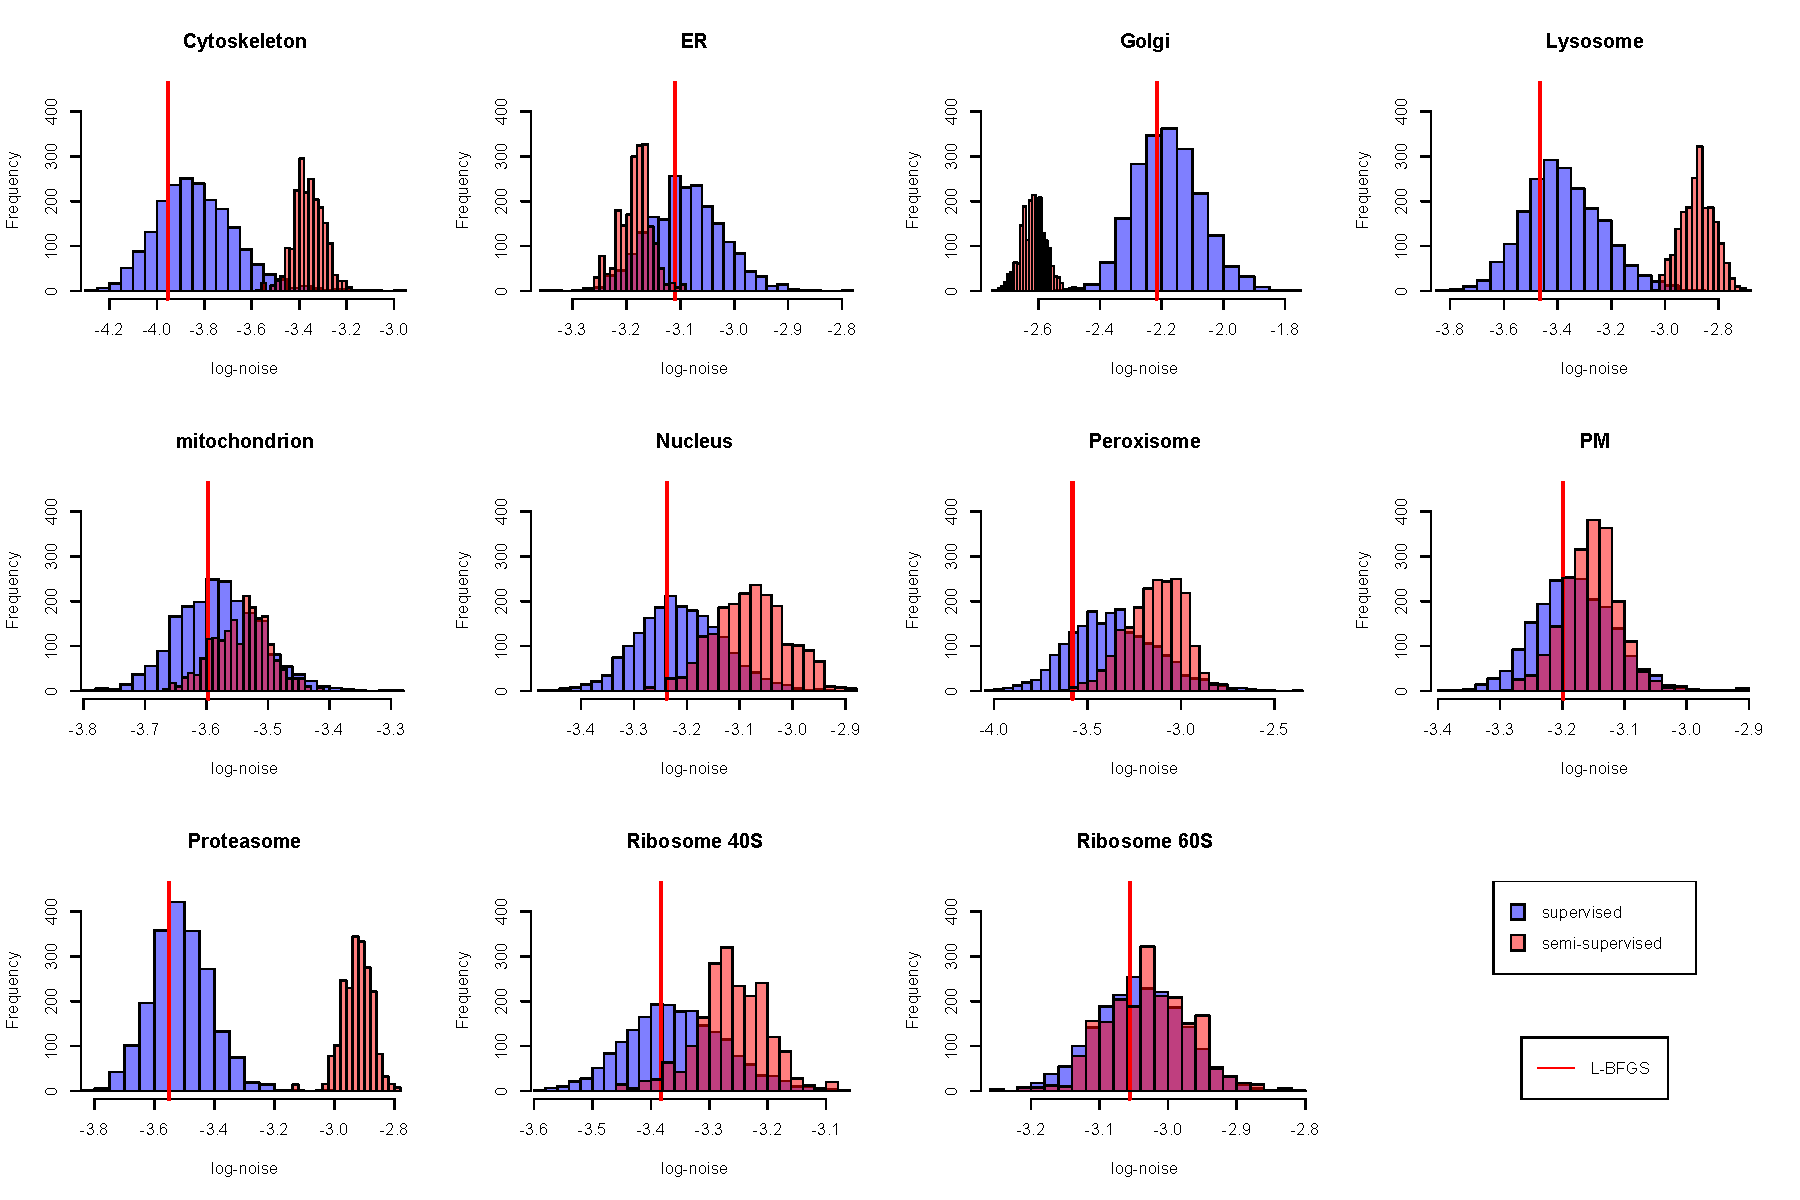
\includegraphics[width= 20cm, height = 12cm]{PosteriorHistTan2009}
      		\centering
      		\caption{ Posterior distributions for the log noise parameter $\sigma^2$.
      		}
      		\label{fig:PosteriorTan}
      	\end{figure}	
      	\item Furthermore, we notice enjoyable shrinkage in the posterior distribution of the noise parameter in the semi-supervised setting. The reduction in variance reduces our uncertainty about the underlying true value of $\sigma_k^2$ for $k = 1,...,K$. 
      	\item  Figure \ref{fig:pcaTan} demonstrates the results of applying our method. Each protein in this PCA plot is scaled according to mean of the Monte-Carlo samples from the posterior localisation probability.
  		}
      	\end{itemize}
      	  
  \begin{figure}[h]
  	\centering
  	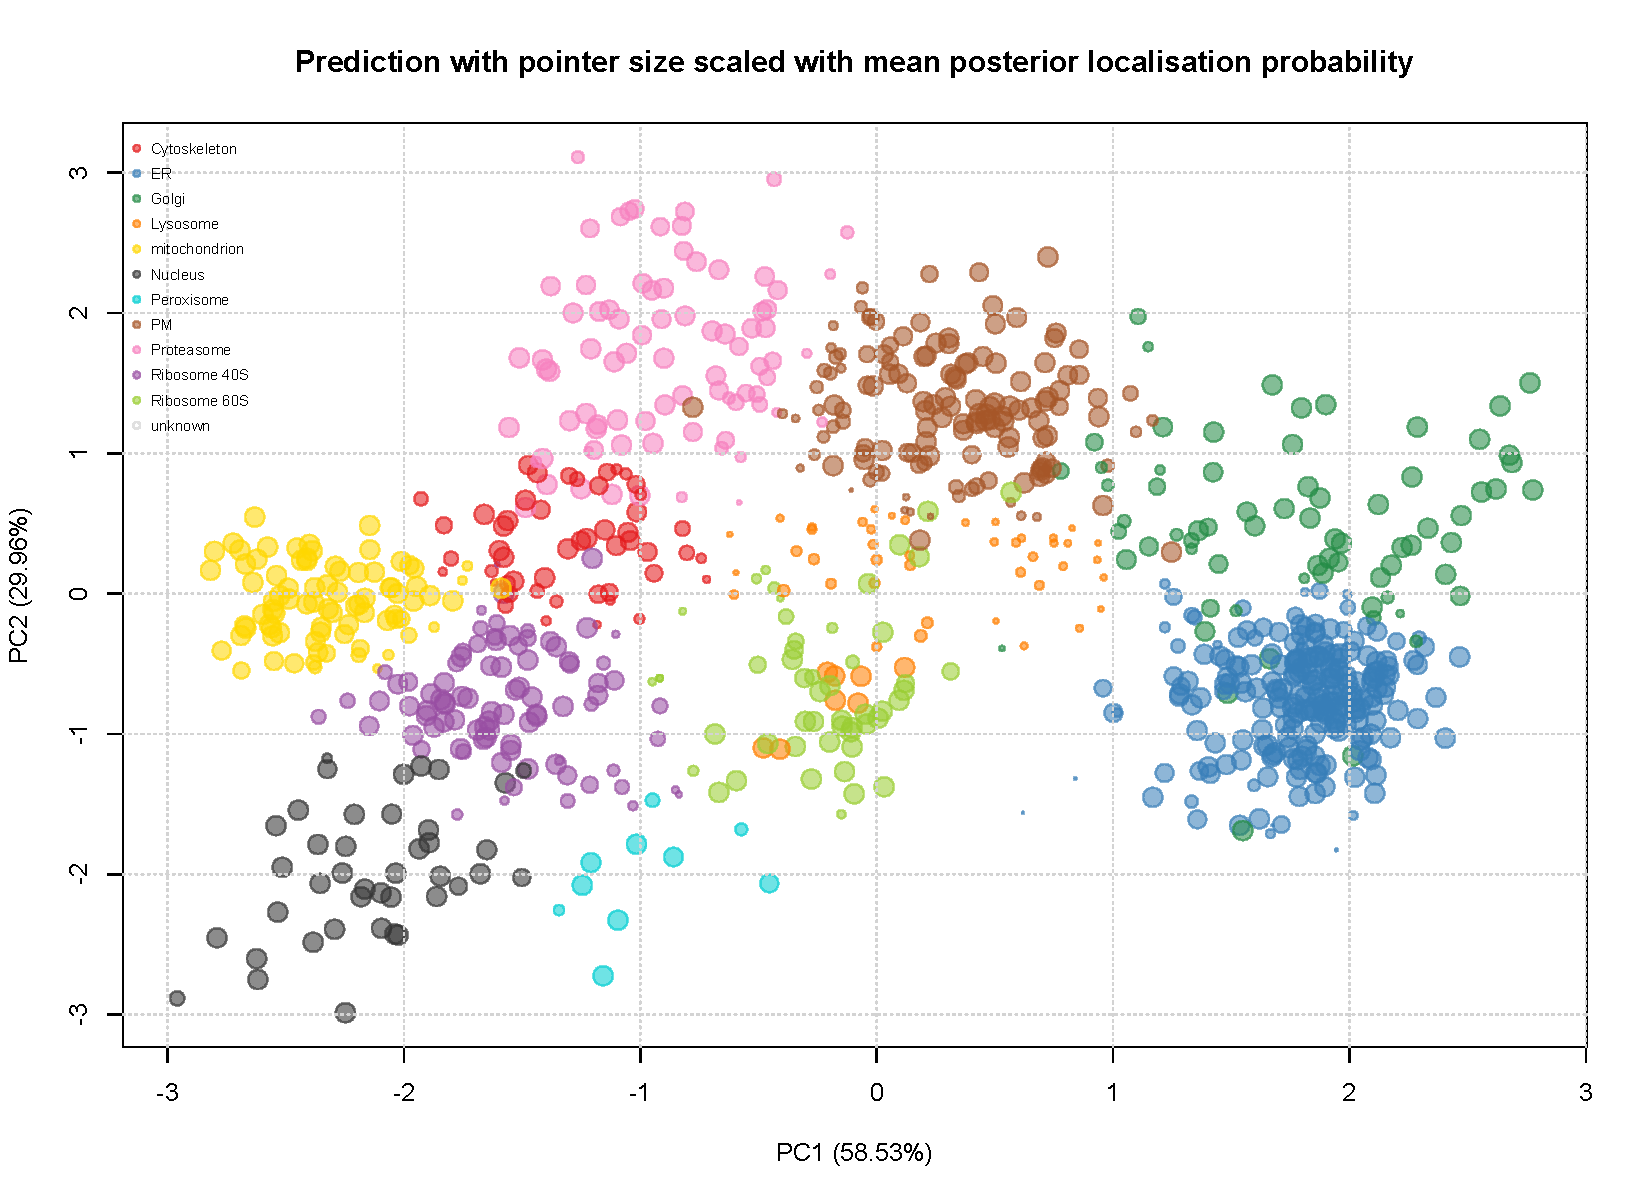
\includegraphics[width= 20cm, height = 12cm]{gpTanpca}
  	\centering
  	\caption{A pca plot for the \textit{Drosophila} data where points, representing proteins, are coloured by the component of greatest probability. The pointer for each protein is scaled with membership probability.
  	}
  	\label{fig:pcaTan}
  \end{figure}
        
     


      \end{block}
      % ----------------------------------------------------------------------------------------

    \end{column} % End of column 2.2

  \end{columns} % End of the split of column 2 - any content after this will now take up 2 columns width



\end{column} % End of the second column

\begin{column}{\sepwid}\end{column} % Empty spacer column

\begin{column}{\onecolwid} % The third column

  % ----------------------------------------------------------------------------------------
  %	CONCLUSION
  % ----------------------------------------------------------------------------------------

  \begin{block}{Results}

         \begin{itemize}
         \small{\item Figure 4 highlights 3 proteins of interest and Figure 5 is a visualization of the probability that these proteins belong to specific classes. 
         \item Figure 5 shows the cases of certain localisation, uncertain localisation between two classes, and no evidence of localisation to any sub-cellular niche.}
         \end{itemize}

  \end{block}
  
          \begin{block}{Conclusion}
          \begin{itemize}
          \small{\item  The proposed Bayesian framework performs consistently with previous methods whilst providing probabilistic information about protein sub-cellular localisations.
          \item This lays the foundation for more complex analysis including full estimation of the posterior assignment probabilities by Gibbs sampling and variational Bayes approximations.
          \item Further investigation is needed to fully exploit the potential of Bayesian models on spatial proteomics data.}
          \end{itemize}
          \end{block}   
          
          
  \begin{block}{Software}
          
              \small{Code to perform the analysis on different datasets and to reproduce the analysis here is provided within the following Bioconductor packages
              \begin{itemize}
              \item MSnbase, pRoloc, pRolocdata
              \end{itemize}
          	}
            \end{block}
          
            % ----------------------------------------------------------------------------------------
  %	REFERENCES
            % ----------------------------------------------------------------------------------------
          
            \begin{block}{References}
            \small{
              \setbeamertemplate{enumerate items}[default]
              \begin{enumerate}
              \item Christoforou, A et al.\textit{A draft map of the mouse pluripotent stem cell spatial proteome} Nat. Commun. (2016)
              \item Breckels, L et al. \textit{Learning from Heterogeneous Data Sources: An Application in Spatial Proteomics} PLoS. Comp. Bio (2016)
              \end{enumerate}
          	}
          
            \end{block}          

  % ----------------------------------------------------------------------------------------
  %	
  % ----------------------------------------------------------------------------------------

  % ----------------------------------------------------------------------------------------
  %	ACKNOWLEDGEMENTS
  % ----------------------------------------------------------------------------------------

  \setbeamercolor{block title}{fg=red,bg=white} % Change the block title color

  \begin{block}{Acknowledgements}

    \small{\rmfamily{Oliver Crook is a PhD student on the Wellcome Trust Mathematical Genomics and Medicine programme and  acknowledges generous funding from the School of Clinical Medicine and the support of the Wellcome Trust. Laurent Gatto is head of the Computational Proteomics Unit and is funded by the BBSRC and the Wellcome Trust.}} \\

  \end{block}

  % ----------------------------------------------------------------------------------------
  %	CONTACT INFORMATION
  % ----------------------------------------------------------------------------------------

  \setbeamercolor{block alerted title}{fg=black,bg=norange} % Change the alert block title colors
  \setbeamercolor{block alerted body}{fg=black,bg=white} % Change the alert block body colors

  \begin{center}
    \begin{tabular}{ccc}
    \end{tabular}
  \end{center}

  % ----------------------------------------------------------------------------------------

\end{column} % End of the third column

\end{columns} % End of all the columns in the poster

\end{frame} % End of the enclosing frame

\end{document}
